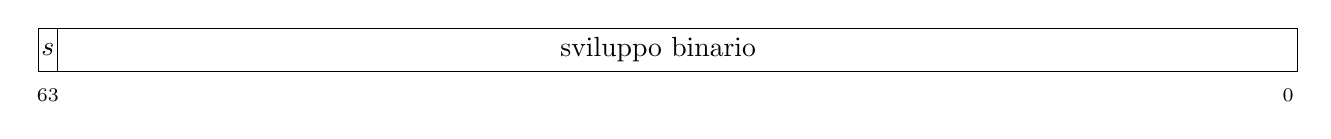
\begin{tikzpicture}[main node/.style={rectangle,draw,inner sep=0.,outer sep=0.}]%
  \pgfmathsetmacro{\xscale}{0.25}
  \pgfmathsetmacro{\yscale}{0.55}
  \draw[draw=black] (0., 0.) rectangle (1. * \xscale, 1. * \yscale);
  \draw[draw=black] (1. * \xscale, 0.) rectangle (64. * \xscale, 1. * \yscale);
  \node at (0.5 * \xscale, 0.5 * \yscale) {$s$};
  \node at (0.5 * \xscale, -0.55 * \yscale) {\scriptsize{$63$}};
  \node at (63.5 * \xscale, -0.55 * \yscale) {\scriptsize{$0$}};
  \node at (31.5 * \xscale, 0.5 * \yscale) {sviluppo binario};
  %\foreach \x in {0,1,...,31}
  %\node[main node] at (\x*\xscale, 0) {0};

  %\foreach \x in {0,1,...,31}
  %\node[main node] at (\x*\xscale, -0.75) {0};
\end{tikzpicture}
